\documentclass{article}
\usepackage{graphicx} % Required for inserting images
\usepackage{url}
\usepackage{amsmath}
\usepackage{subcaption}

\title{A Machine Learning Classification Model for Gold-Binding Peptides}
\author{Ali Ahmadi Esfidi}
\date{May 2025}

\begin{document}

\maketitle

\section{Gold-Binding Peptides}
Gold‐binding peptides are short chains of amino acids (typically 5–20 residues) that have a natural affinity for gold surfaces or nanoparticles. They are identified or designed so that specific residues (often cysteine, histidine, or aromatic amino acids) coordinate with gold atoms, allowing the peptide to stick strongly and specifically to gold.\footnote{\url{https://pmc.ncbi.nlm.nih.gov/articles/PMC10337651/}}

\subsection{Usage}
\begin{enumerate}
  \item \textbf{Nano‐templating \& Nanofabrication.} Peptides guide the formation of gold nanowires, rods, or particles with controlled size and shape, serving as a “molecular mold” for electronic or optical devices.\footnote{\url{https://pubs.rsc.org/en/content/articlepdf/2023/ra/d3ra04269c}}
  \item \textbf{Biosensing \& Diagnostics.} When immobilized on electrodes or sensor surfaces, gold‐binding peptides can capture target biomolecules (e.g., antibodies) in a precise orientation, improving sensitivity for medical assays.\footnote{\url{https://pmc.ncbi.nlm.nih.gov/articles/PMC9918321/}}
  \item \textbf{Targeted Drug Delivery \& Imaging.} Conjugating drugs or imaging agents to gold nanoparticles via these peptides allows for targeted delivery and enhanced imaging contrast in cancer or inflammatory disease models.\footnote{\url{https://www.sciencedirect.com/science/article/abs/pii/S0378517324011542}}
  \item \textbf{Surface Functionalization.} They enable simple, one‐step coating of gold surfaces with proteins or other functional polymers, useful in creating antifouling coatings or bioactive interfaces.
\end{enumerate}

\subsection{Intensity}
In spot‐array binding assays, each 10‐residue peptide is immobilized on a solid support and exposed to gold nanoparticles. The \emph{intensity} is defined as the optical (colorimetric) signal measured at each peptide spot, proportional to the amount of bound nanoparticles. Peptides with stronger binding produce darker spots (higher intensity), whereas weak or non‐binding sequences yield lighter spots (lower intensity).

In the dataset of Janairo \emph{et al.}, each of the 1\,720 unique 10‐mer peptides was assigned an intensity value based on the median image‐analysis readout from Tanaka \emph{et al.}'s screen. To classify peptides into binders and non‐binders, the median intensity of the entire set, denoted \(I_{\mathrm{med}}\), was used as the threshold:
\[
I_{\mathrm{med}} = 207{,}500 \quad\text{(arbitrary units)}.
\]
Peptides were then dichotomized into two classes:
\begin{align*}
\text{Class A (strong binders)} &: I > I_{\mathrm{med}}, \\
\text{Class B (weak/non‐binders)} &: I \le I_{\mathrm{med}}.
\end{align*}

Thus, the intensity values (in arbitrary units) provide a relative measure of each peptide’s adsorption of gold nanoparticles under the standardized assay conditions.


\section{Formulation of Problem}
\begin{itemize}
    \item \textbf{Input:}\begin{enumerate}
        \item \textbf{Peptide sequence:} A string of ten amino‐acid letters.

        \item \textbf{Derived features:} Each sequence is converted into a fixed-length numeric vector, so that the model can process it.
    \end{enumerate}

    \item \textbf{Output:} A binary prediction for each input sequence:
    \begin{itemize}
        \item “Strong binder” (class A) if the model believes the peptide’s binding intensity would exceed the threshold set by the median of all measured intensities.
        \item “Weak/non-binder” (class B) otherwise.
    \end{itemize}
\end{itemize}
\subsection{Mathematical Presentation}
\begin{enumerate}
    \item Peptide Sequences:    \[S = \{s_i\},\quad s_i \in \mathcal{A}^{10}\]

    \item Feature Mapping:    \[\forall s_i \in S, \quad \Phi(s_i) = x_i \in \mathbb{R}^d\]
    
    \item Binding Intensities:    \[I = \{I_i\}_{i=1}^N,\quad I_i \in \mathbb{R}_{\ge0},\]

    \item Classification Labels:   \[y_i = 
    \begin{cases}
      A, & I_i > T,\\
      B, & I_i \le T,
    \end{cases}
    \quad T = \mathrm{median}\bigl(\{I_i\}\bigr)\]

    \item Prediction Function: \[
    \forall s_i \in S, \quad
    f(\Phi(s_i)) = \hat y_i \in \{A,B\}
    \]
\end{enumerate}

\subsection{Assumptions}
\begin{enumerate}
  \item All peptides have fixed length 10.
  \item Median intensity threshold $T$ meaningfully separates strong vs.\ weak binders.
  \item Samples are independently and identically distributed.
\end{enumerate}

\section{Dataset}
Dataset comprises 1,720 peptide sequences, which we classify as A or B based on their intensity values.\footnote{\url{https://pubs.acs.org/doi/suppl/10.1021/acsomega.2c00640/suppl_file/ao2c00640_si_001.pdf}}

\subsection{Distribution}
It’s important to confirm class balance before training classifiers, as imbalanced datasets can introduce bias. 

The class sizes are nearly identical; exact count: \textbf{861} for Class A and \textbf{859} for Class B.

However, as illustrated in the violin plot and histogram in Figure 1, Class A peptides are high-intensity binders with intensity values concentrated around 250,000. Class B peptides, conversely, exhibit lower intensity values, ranging widely from nearly 0 to 200,000, and display a prominent left tail.

\begin{figure}[h!]
    \centering
    \begin{subfigure}[b]{0.45\textwidth}
        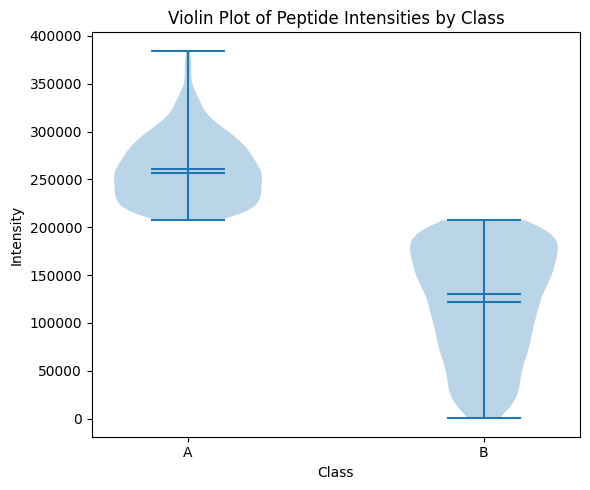
\includegraphics[width=\textwidth]{images/1.png}
        \label{fig:subfig1}
    \end{subfigure}
    \hfill % Adds horizontal space between the subfigures
    \begin{subfigure}[b]{0.45\textwidth}
        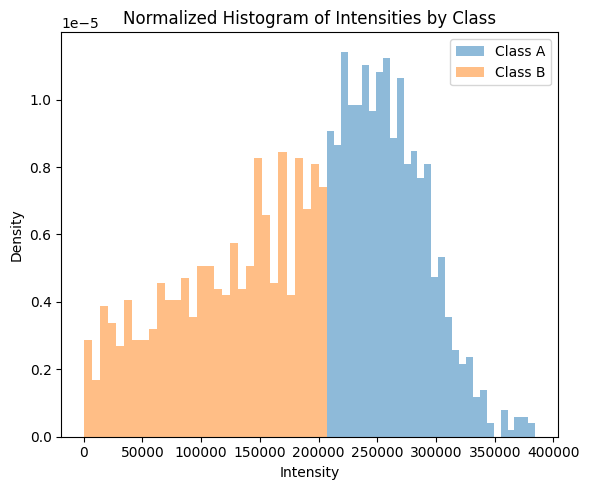
\includegraphics[width=\textwidth]{images/2.png}
        \label{fig:subfig2}
    \end{subfigure}
    \caption{Overall caption for both images.}
    \label{fig:two_images}
\end{figure}

\section{Related Work}
As part of his lecture series, Jose Isagani B. Janairo presents a practical workflow for classifying gold-binding peptides that elegantly demonstrates end-to-end machine-learning in R: starting with raw amino-acid sequences, deriving ten physicochemical descriptors via Kidera factors, and organizing those into a labeled dataset; next, stratified train–validation splitting and 10-fold cross-validation to tune and compare multiple classifiers (logistic regression, decision trees, k-nearest neighbors, SVMs with various kernels, and a neural network); then refining the best performer—a radial-basis SVM—by selecting only the most informative descriptor subset; and finally, assessing generalization on hold-out data and employing permutation-based feature importance to reveal which peptide properties most strongly drive gold-binding predictions, all accompanied by clear visualizations of model performance and variable rankings.

On a macOS environment, the code was executed and produced results (Table 1) consistent with the related lecture (Accuracy: 0.8019).

\begin{table}[h!]
\centering
\begin{tabular}{|c|c|c|}
\cline{2-3}
\multicolumn{1}{c|}{} & \multicolumn{2}{c|}{\textbf{Reference}} \\
\cline{2-3}
\multicolumn{1}{c|}{} & \textbf{A} & \textbf{B} \\
\hline
\textbf{Prediction A} & 175 & 45 \\
\textbf{Prediction B} & 40 & 169 \\
\hline
\end{tabular}
\caption{Confusion Matrix}
\end{table}

Also Table 2 reports the permutation-based importance of each Kidera factor (KF1–KF10) for the final radial‐basis SVM, together with uncertainty bounds and the baseline increase in classification error when that feature is shuffled.

\begin{table}[h!]
\centering
\label{tab:feature_importance}
\begin{tabular}{|c|c|c|}
\hline
\textbf{feature} & \textbf{importance} & \textbf{permutation.error} \\
\hline
KF4 & 1.446512 & 0.2408985 \\
KF2 & 1.395349 & 0.2323780 \\
KF3 & 1.395349 & 0.2323780 \\
KF9 & 1.306977 & 0.2176607 \\
KF10 & 1.158140 & 0.1928737 \\
KF5 & 1.148837 & 0.1913246 \\
KF7 & 1.144186 & 0.1905500 \\
KF6 & 1.130233 & 0.1882262 \\
KF1 & 1.000000 & 0.1665376 \\
KF8 & 1.000000 & 0.1665376 \\
\hline
\end{tabular}
\caption{Feature Importance}
\end{table}

In practice, this tells you that the model heavily relies on KF4, KF2, and KF3—disrupting these degrades performance the most—whereas KF1 and KF8 contribute almost nothing to gold‐binding predictions in the final SVM.

\end{document}
